\documentclass{beamer}

\usetheme{Warsaw}
\usecolortheme{orchid}
%\useoutertheme{miniframes}
%\useinnertheme{rounded}
\usepackage{subcaption}

\usepackage{multimedia}

\usepackage{amssymb}
\usepackage{amsmath}
%\usepackage{svg}
\usepackage{float}


\usepackage{default}

\begin{document}

\begin{frame}
\frametitle{\textit{Michael Reed}, UNCG Undergraduate}
\begin{itemize}
	\item Member: \textit{American Institute of Aeronautics and Astronautics}
	\item Member: \textit{American Mathematical Society}
	\item Collaborating with Dr. Vladimir Golubev (ERAU, AFOSR) on \textit{Multi-disciplinary Design Optimization of Synthetic Jet Actuators for Transitional Boundary Layer Separation Control}
	\item First gained interest in \textbf{Modular Forms} exactly one year ago.
	\item \textbf{Research Interest}: Investigate the occurrence of doubly-periodic vortex soliton solutions of coupled nonlinear hyperbolic partial differential equations.
	\item \textbf{Research Interest}: Arithmetic on groves of planar binary trees using the Loday-type dendriform dialgebra. 
	\item \textbf{Research Interest}: Symbolic computation and term rewriting using abstract syntax trees for expressions.
\end{itemize}
\end{frame}
\begin{frame}
\frametitle{\textit{Michael Reed}, Toroidal Vortex Expulsion}
\begin{figure}[ht]\centering
	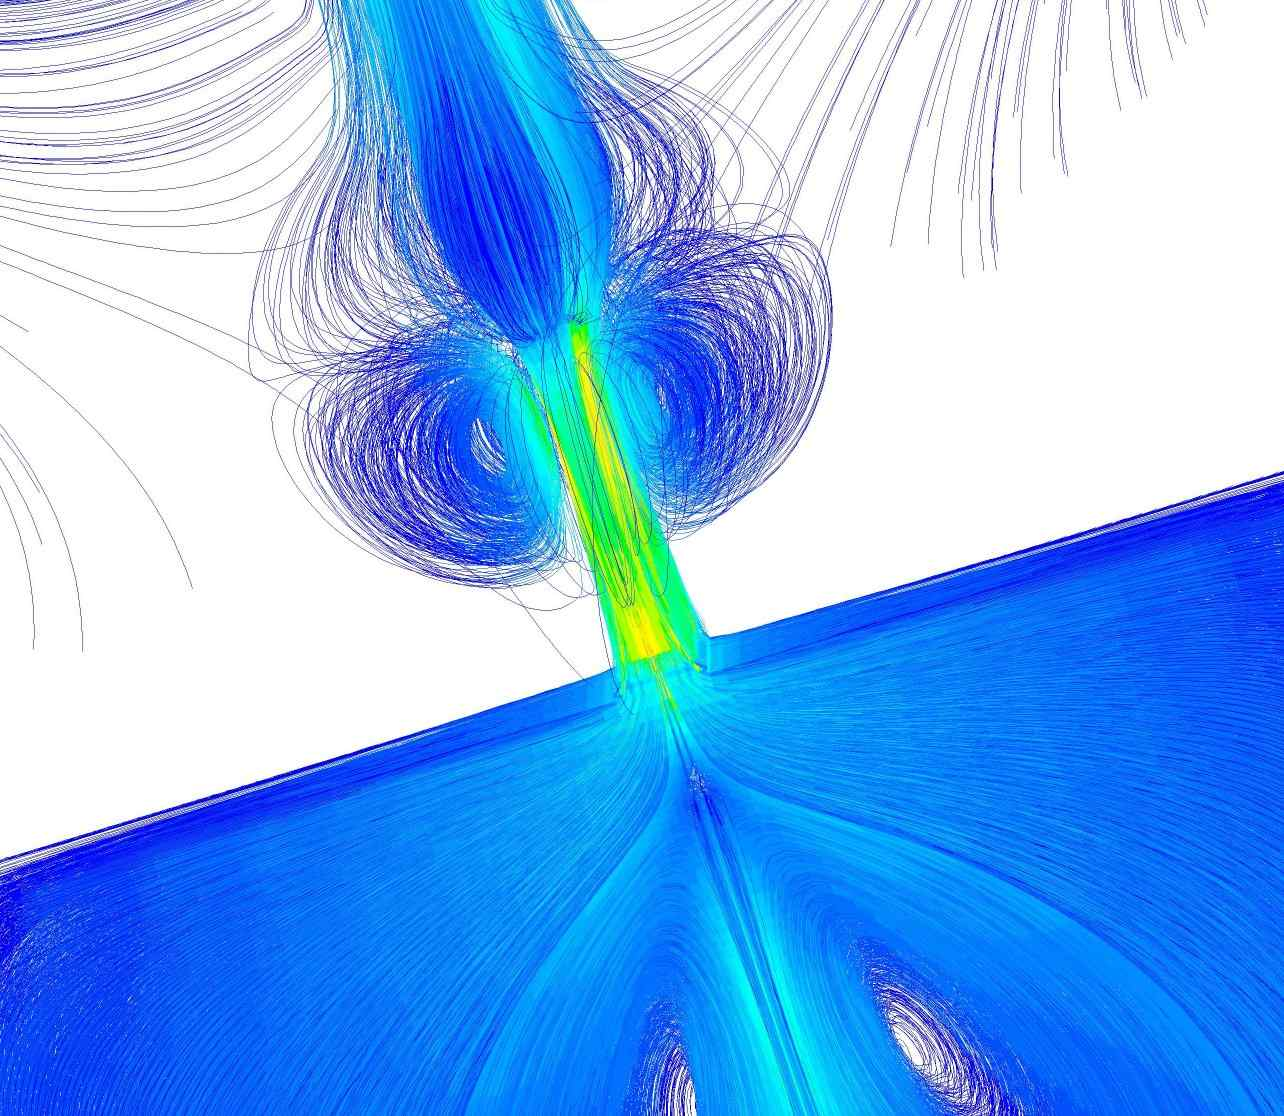
\includegraphics[width=8cm]{kev.jpg}
	\caption{Vena contracta visible near orifice of asymmetric flow synthetic jet actuator, 3D Reynolds Averaged Navier-Stokes PDE.}
\end{figure}
\end{frame}


\end{document}
